\vspace{-0.1cm}
\begin{wraptable}[8]{r}{0.53\textwidth}
\vspace{-0.1cm}
\centering{
  \begin{tabular}{|l|r|r|p{0.1\textwidth}|}
    \hline
          & HAP                     & experiment          & ref.\\
    \hline 
    $\KB$ & $11 \pm 2.5$ \kBT       & 10 \kBT               & \cite{Naetal15,VeBrPa15,NAGLE2000159,PhysRevLett.113.248102}\\
    \hline 
    $\KA$ & $34$ \kBT \; nm$^{-2}$  & 30--40 \kBT nm$^{-2}$ & \cite{Nagle17, Nagle17-2}\\
    \hline 
    $\KTH$ & $12$ \kBT \; nm$^{-2}$ & 10 \kBT nm$^{-2}$     & \cite{KUZMIN2005, KoNa15} \\ \hline
  \end{tabular}
}
  \vspace{-8pt}
\caption{\label{tab:moduli} \footnotesize Comparision of values elastic
  moduli from the experimental literature and values derived by HAP
  simulation.} 
\end{wraptable}
\section{Preliminary work}
\label{sec:preliminary_work}
PIs RR and YNY started work on HAP modeling with Szu-Pei Fu (then PI YNY's student and now PI RR's postdoc) and collaborators in 2017. 
%
%
%The HAP project was initiated in 2017 by PI RR and YNY. The lead author
%on our first paper~\cite{Fu2018_SIAM} was Szu-Pei Fu, who was PI YNY's
%PhD student and is currently a postdoc with PI RR. The collaboration
%involved theoretical work and simulation. The theoretical work included
%model development, proving the first variation formula~\eqref{stress}
%and force-free law, and an energy-based uniqueness theorem for the
%exterior domain problem~\eqref{SL}. 
%Coauthors Andreas Kl\"ockner
%(Computer Science, UIUC, NSF CAREER \#1654756) and his PhD student Matt
%Wala provided their Quadrature by Expansion, or QBX algorithm and Fu ran
%simulations on NJIT clusters.
%
\begin{wraptable}[11]{l}{0.43\textwidth}
\centering{
  \begin{tabular}{|l|l|l|l|}
    $n$   & (rel.~err.)$_F$
    &  (rel.~err.)$_G$ \\
    \hline
% 32   &   4.07466     &   1.56437\\
% 64   &   0.24664     &   0.03476\\
% 128  &   0.00063     &   0.00006\\
  32  & $4.07 \times 10^{+0}$ & $1.56 \times 10^{+0}$ \\
  64  & $2.47 \times 10^{-1}$ & $3.48 \times 10^{-2}$ \\
  128 & $6.30 \times 10^{-4}$ & $6.00 \times 10^{-5}$ 
  \end{tabular}}
\vspace{-5pt}
\caption{\label{tab:spectral_force} 
\footnotesize  Relative numerical errors (rel.~err.)$_F = \max_{i}
  \|\mathbf{F}_i-\mathbf{F}_i^{\text{exact}}\|/\|\mathbf{F}_i^{\text{exact}}\|$
  and (rel.~err.)$_G = \max_{i}
  \|\mathbf{G}_i-\mathbf{G}_i^{\text{exact}}\|/\|\mathbf{G}_i^{\text{exact}}\|$
  for force and torque respectively as a function of number of grid
  points $n$ per particle.  The data is for $N = 5$ particles; two of
  the particles are nearly touching at a distance 1\% of particle
  diameter.} 
\end{wraptable}
The results are summarized in \cite{Fu2018_SIAM}, where
small particle-number simulations successfully demonstrated gradient-driven self-assembly of
amphiphilic particles into two-dimensional micelles and bilayer membranes with realistic values of
the model parameters:  decay length $\rho=2.5$ nm (based on measurements of
hydrophobic attraction between surfactant-coated
membranes~\cite{Eriksson1989, Lin2005, Parsegian, Israelachvili80}),
particle diameter 2.0 nm (the physical monolayer thickness, 2.0 nm~\cite{Boal}),
and interfacial tension $\gamma = 4$ pN nm$^{-1}$ based on
measurements for single-component bilayer lipid
membranes~\cite{GarciaSaez, KUZMIN2005, Petelska2012, Jackson2016}.

%\begin{wrapfigure}[]{r}{0.5\textwidth}
%  \centering{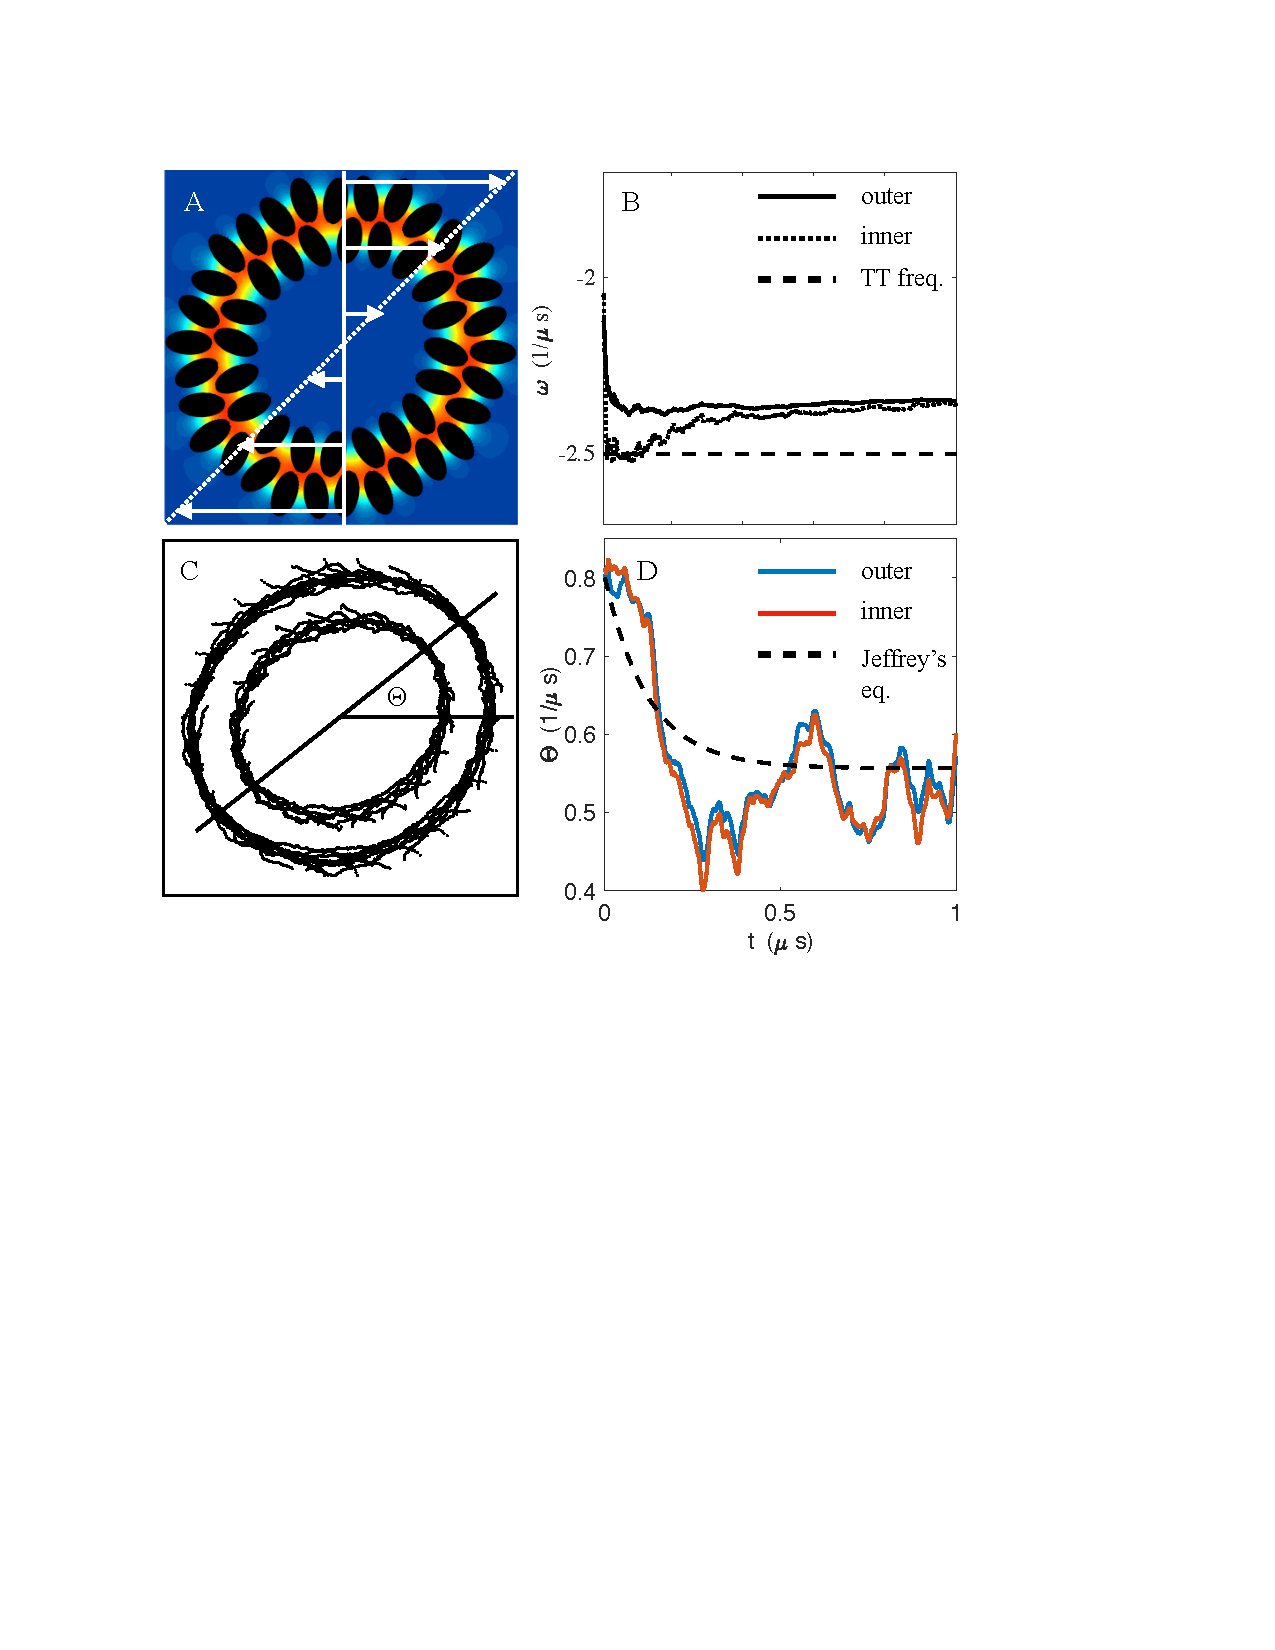
\includegraphics[width=0.5\textwidth]{Figures/TankTreading.pdf}}
%  \vspace{-25pt}
%  \caption{\label{fig:tank_treading} \footnotesize
%    Panel A shows water activity and flow direction for  a two-dimensional
%    particle-based vesicle in a shear flow; $\mu  = 1$ mPa s,
%    $\dot{\gamma} = 0.5$ $\mu$s$^{-1}$. Panel B plots the
%    mean angular velocities for the outer leaflet and the inner
%    respectively.  Panel C shows that the trajectory of the particle
%    centers forms two ellipses with well-defined inclination angle
%    $\Theta$. Panel D shows the evolution of the inclination angle.
%    Panels B and D share the same time axis.}
%\end{wrapfigure}
The paper \cite{Fu2018_SIAM} considered three types of simulations. The first measured bending by
loading a partially clamped planar bilayer. The second used a harmonic
bond to dilate a circular bilayer. The third measured tilt using a decay
equation from~\cite{KUZMIN2005}. These simulations isolated three of the
five deformations of~\eqref{ansatz3}, enabling us to read off elastic
moduli from simulation data. The results agreed remarkably well with the
values reported in the experimental literature (Table~\ref{tab:moduli}).
The agreement is underscored by the fact that the two main HAP
parameters, $\gamma$ and $\rho$, were assigned physical values from the
outset rather than being tuned to fit data. 

PIs BQ, RR and YNY initiated a collaboration in Summer 2020 to
develop the hydrodynamic model of \S\ref{subsec:specific_aim_3}.  To
date, we have written solvers for the two-dimensional boundary integral
formulations of~\eqref{SL} and~\eqref{eq:stokes} that achieve
third-order accuracy up to the boundary. The specialized reciprocal
identity~\eqref{eq:reciprocal} gives spectral accuracy for force and
torque (Table~\ref{tab:spectral_force}).
\begin{wrapfigure}[]{r}{0.5\textwidth}
  \centering{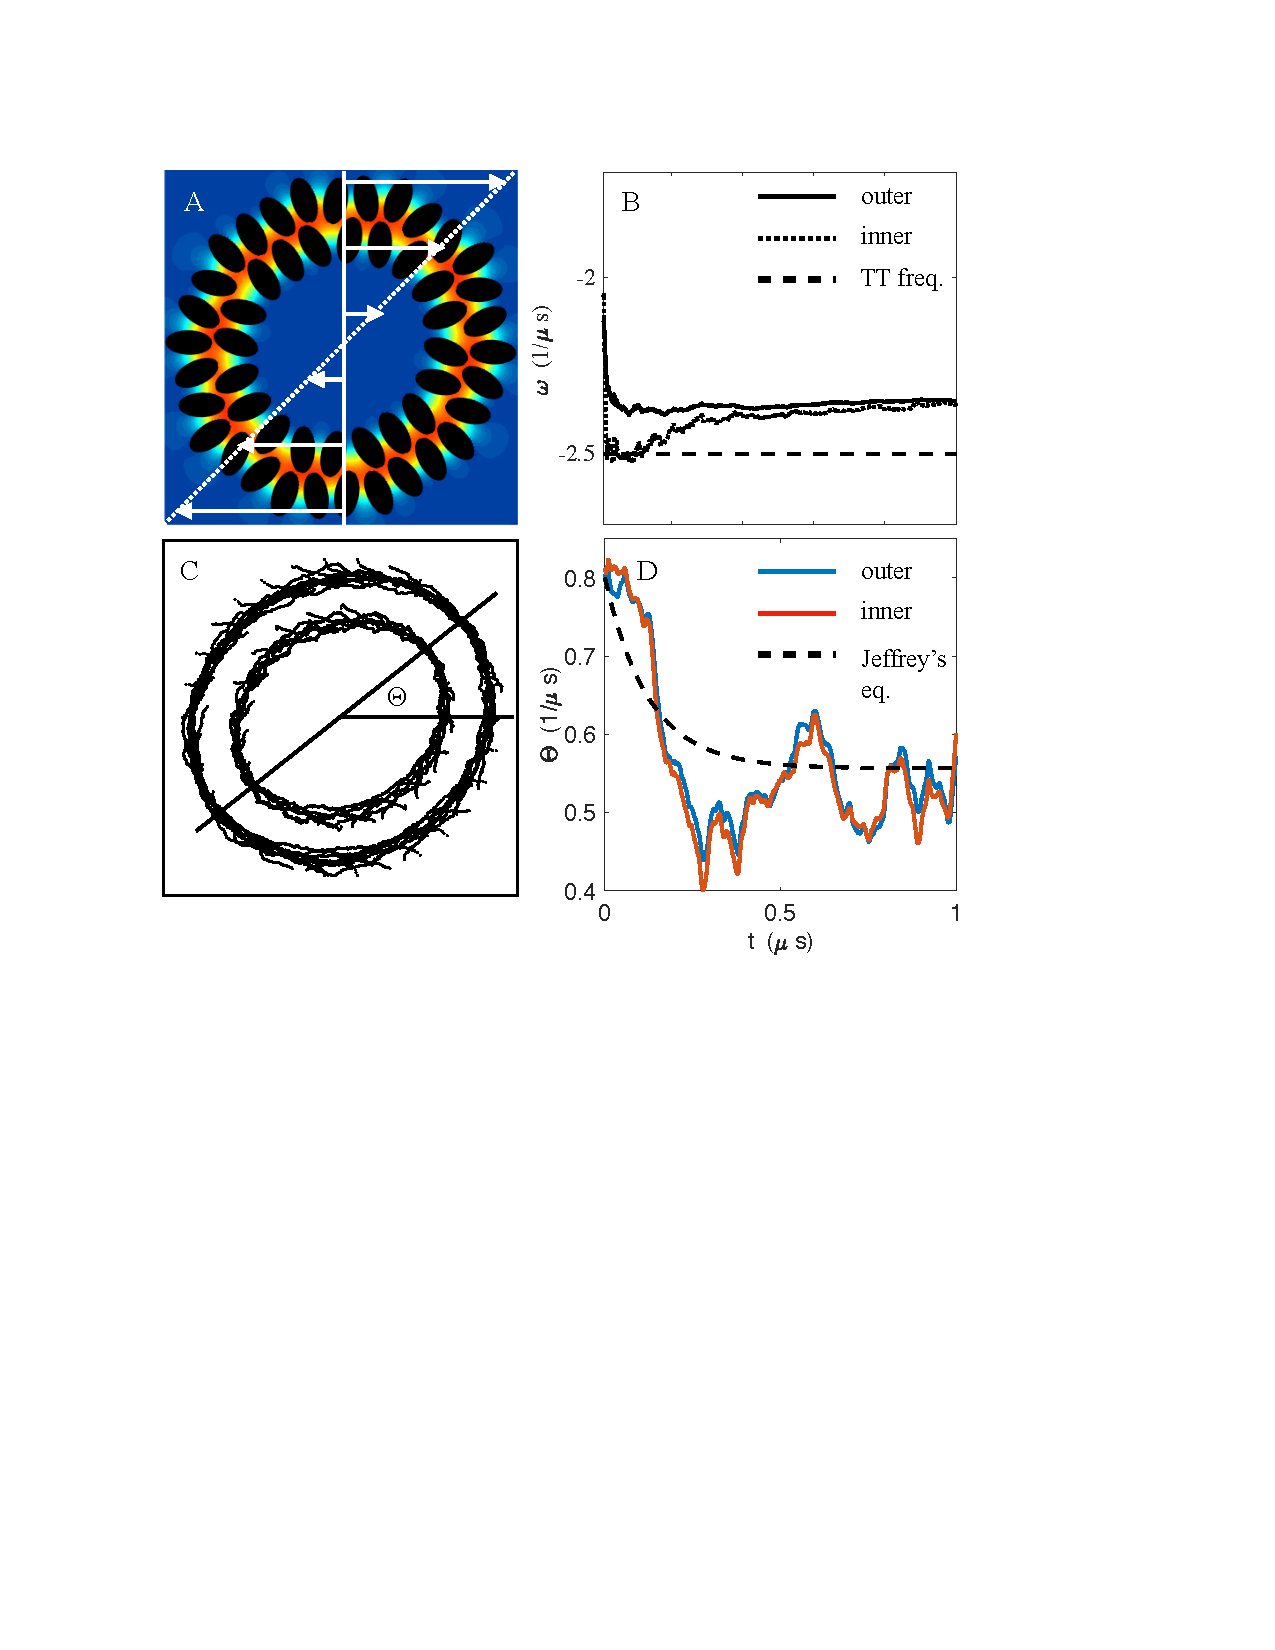
\includegraphics[width=0.5\textwidth]{Figures/TankTreading.pdf}}
  \vspace{-25pt}
  \caption{\label{fig:tank_treading} \footnotesize
    Panel A: A two-dimensional
    particle-based vesicle in a shear flow (arrows); $\mu  = 1$ mPa s,
    $\dot{\gamma} = 0.5$ $\mu$s$^{-1}$. The color coding is for HAP. Panel B: The
    mean angular velocities for the outer leaflet and the inner
    respectively.  Panel C: The trajectory of the particle
    centers forms two ellipses with well-defined inclination angle
    $\Theta$. Panel D: The evolution of the inclination angle.
    Panels B and D share the same time axis.}
\end{wrapfigure}

We have simulated two-dimensional vesicles in shear flow
$\mathbf{u}_{\infty} = \dot{\gamma} x_2 \mathbf{i}_1$ with shear rate
$\dot{\gamma}$,
%(The symbol shear rate is unrelated to interfacial tension.)
and the particle-based system mimics the behavior observed in continuous
vesicles~\cite{torres-sanchez_millan_arroyo_2019,
mahapatra_saintillan_rangamani_2020, Steigmann99, C6SM02452A}. The basic
pattern is that the vesicle bilayer approaches a steady tank-treading
ellipse (Figure~\ref{fig:tank_treading}C). We analyzed the simulation
data in the context of theoretical work on
tank-treading~\cite{Finken2008, PhysRevLett.106.158103}.
Jeffrey's equation predicts a
tank-treading frequency $-\dot{\gamma}/2$ (dashed line in
Figure~\ref{fig:tank_treading}B). In the particle simulation, the
tank-treading frequency corresponds to the mean of the particle angular
velocities, and these approach a value within 7\% of the theoretical
prediction (dotted and solid curves in Figure~\ref{fig:tank_treading}B).
In the low viscosity-contrast regime of our simulation, Jeffrey's
equation predicts a decrease in the ellipse's inclination angle $\Theta$
and our particle-based simulation follows this prediction
(Figure~\ref{fig:tank_treading}D), albeit with some higher frequency oscillation
coming from particle reorganization.

Analyzing for any underlying constitutive laws, the particles reorganize
so that there is an initial increase and then plateauing of vesicle
circumference. As is the case with real lipid bilayer membranes, the
particle collection permits a small amount of stretching. The
theoretical calculations give an increase of length by 3.6\% and this amount
agrees with our measured increase in length. The simulations also
suggest that the particle system behaves as a semipermeable
vesicle~\cite{323e9a2f0c58487ea82518d7a1f96485, YAO2017728}.

\begin{wrapfigure}[11]{l}{0.22\textwidth}
  \centering{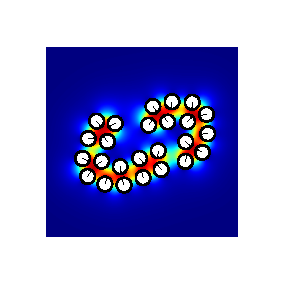
\includegraphics[width=0.22\textwidth]{Figures/PW_fig5.pdf}}
  \caption{\label{fig:flow_rupture} \footnotesize Rupture of a
  two-dimensional vesicle at large shear rates.}
\end{wrapfigure}
The above considerations further justify using the particle-based model
to study material properties as outlined in
\S\ref{subsec:specific_aim_1}. Furthermore, the particle system allows
for intermonolayer slip~\cite{SHKULIPA2005823, ShkulipaThesis}. In
Figure \ref{fig:tank_treading}B, the inner angular velocity is slightly
less than the outer angular velocity. Intermonolayer slip enters
zero-thickness membrane models as a velocity jump boundary condition
\cite{schwalbe_vlahovska_miksis_2010}, for example, but in the present
model, it is a consequence of monolayer independence. For large shear
rates, viscous forces exceed the hydrophobic attraction to the point that
the vesicle ruptures. The flow carries away segmented membrane patches
(Figure \ref{fig:flow_rupture}). 

In conclusion, the HAP model accurately mimics the behavior of continuous
membranes, while at the same time capturing the
reconnection during the topological change of 
lipid molecules on the scales of membrane thickness,
overcoming one of the long-standing challenges of continuum modeling.

%%%%%%%%%%%%%%%%%%%%%%%%%%%%%For Specific Aim 3
%The background flow enters by replacing the third equation in \eqref{eq:stokes} 
%with the condition $(\mathbf{u} -\mathbf{u}_{\infty})(\mathbf{x}) 
%\to \mathbf{0}$ as $|\mathbf{x}| \to \infty$. To incorporate the far-field flow, 
%and using the representation 
%\begin{align}
%\label{PowerMiranda}
%  {\bf u} = {\bf u}_{\infty} + K\boldsymbol{\eta} + 
%    \sum_{i=1}^N S(\cdot, {\bf a}_i) {\bf F}_i + 
%                 R(\cdot, {\bf a}_i) {\bf G}_i.
%\end{align}
%The symbols $S$ and $R$ are Stokeslets and rotlets supported at the respective
%particle centers \cite{leal_2007} and $K\boldsymbol{eta}$ is a layer potential for the
%unknown density function $\boldsymbol{\eta}.$ The
%representation~\eqref{PowerMiranda} automatically satisfies all
%equations, with the exception of the rigid motion conditions. The rigid
%motion conditions follow by requiring the viscous stress vanishes across
%the particle boundaries.

%\begin{wrapfigure}[13]{l}{0.30\textwidth}
%\centerline{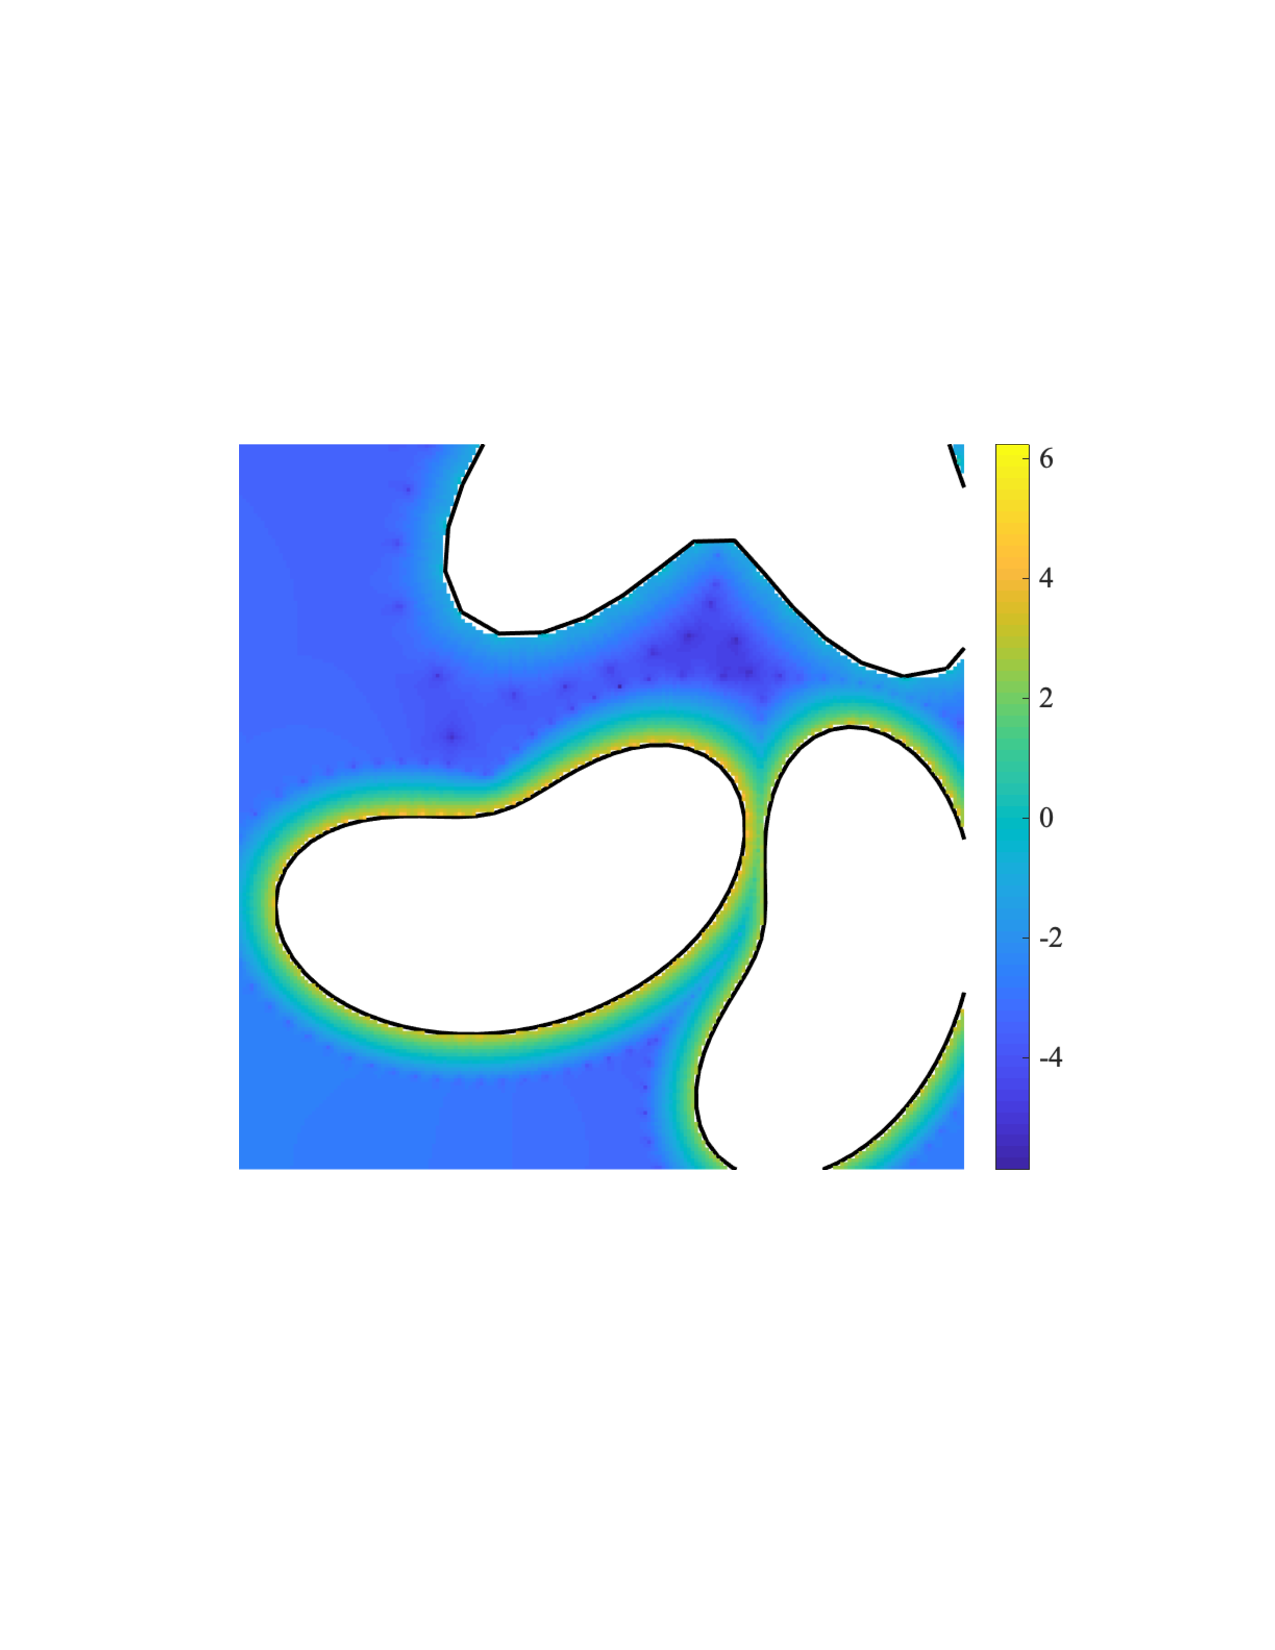
\includegraphics[width=0.30\textwidth]{figures/BIError.pdf}}
%  \vspace{-8pt}
%\caption{
%\label{fig:bierror}  
%\footnotesize The false color map shows how numerical quadrature of
%  layer potentials loses accuracy near the particle boundaries.  The
%  color bar is for $\log_{10}.$}
%\end{wrapfigure}
%\textbf{Novel reciprocal identities.} 
%The force and torque formulas~\eqref{forceandtorque} require the
%hydrophobic stress along the particle boundaries. Unfortunately,
%standard quadrature formulas to estimate $\nabla u$ on the particle
%boundaries introduces large amounts of quadrature error
%(Figure~\ref{fig:bierror}). Therefore, it is useful to devise reciprocal
%identities for the force and torque on body $i$ that does not
%require integration along body $i$. One identity, that we have proved,
%is
%\begin{align}
%    \label{eq:reciprocal}
%{\bf F}_{\text{hydro},i} = \sum_{j \neq i} \int_{\partial P_i}
%[\boldsymbol{\sigma}_{ij} + \boldsymbol{\sigma}_{ji}]\boldsymbol{\nu}\,\dif S,\quad
%{\bf G}_{\text{hydro},i} = \sum_{j \neq i} \int_{\partial P_i} ({\bf
%  x}-\mathbf{a}_i) \times [\boldsymbol{\sigma}_{ij} +
%  \boldsymbol{\sigma}_{ji}]\boldsymbol{\nu}\,\dif S, 
%\end{align}
%for $i=1,\ldots,N$. Here, $u_i$ is the solution of the screened Laplace
%equation when only the contribution from particle $i$ is considered and
%$\boldsymbol{\sigma}_{ij} = \rho^{-1} u_iu_j {\bf I} + \rho(\nabla u_i
%\cdot \nabla u_j {\bf I} - 2 \nabla u_i \otimes \nabla u_j)$.
%Because of the double layer potential jump relations, \eqref{eq:reciprocal} 
%does not require knowledge of $\nabla u$ on the particle boundary, and this
%is enormously beneficial for calculating force and torque.



%\subsection{Two-dimensional vesicle hydrodynamics in shear flow} 
%The motion of vesicles in shear flow is an important problem in the
%applied mathematics because simulations can reveal mechanical
%properties of membranes and lead to an enhanced understanding of
%deformable particle laden flows \cite{Sinha15}. 
%
%
%\begin{wrapfigure}[10]{r}{0.2\textwidth}
%\centerline{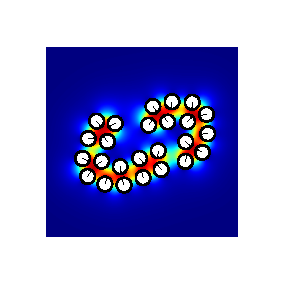
\includegraphics[width=0.2\textwidth]{figures/PW_fig5.pdf}}
%\vspace{-8pt}
%\caption{\label{fig:rupture} \footnotesize Rupture of tank-treading vesicle under strong shear flow.}
%\end{wrapfigure}
%
%To implement a vesicle in shear flow in the context of hydrophobic
%potentials and mobility problem, we consider a shear flow in the
%far-field $\mathbf{u}_{\infty} = Uy\mathbf{i}_x$ in the direction of the
%$x$-axis (Figure \ref{fig:tanktreading}A). As illustrated in Figure
%\ref{fig:tanktreading}, the particle based approach supports
%inter-leaflet slip, and this can be used to determine inter-leaflet and
%in-plane shear viscosities. 
%
%This field satisfies the linear Stokes system but does not give rise to a rigid motion at the particle interfaces. 
%To have a rigid motion, we change variables $\mathbf{u} = \tilde{\mathbf{u}}+ \mathbf{u}_{\infty}$ and 
%for the new field $\tilde{\mathbf{u}}$ vanishing at infinity we let 
%$\tilde{\mathbf{u}}|_{\partial P_i} = \mathbf{v}_i + \boldsymbol{\omega}_i \times (\mathbf{x} - \mathbf{a}_i)$ 
%where $(\mathbf{v}_i,\boldsymbol{\omega}_i)$ are the unknown translation and angular velocities of the 
%$i$th particle $P_i.$  
%
%\begin{wrapfigure}[17]{l}{0.4\textwidth}
%\centerline{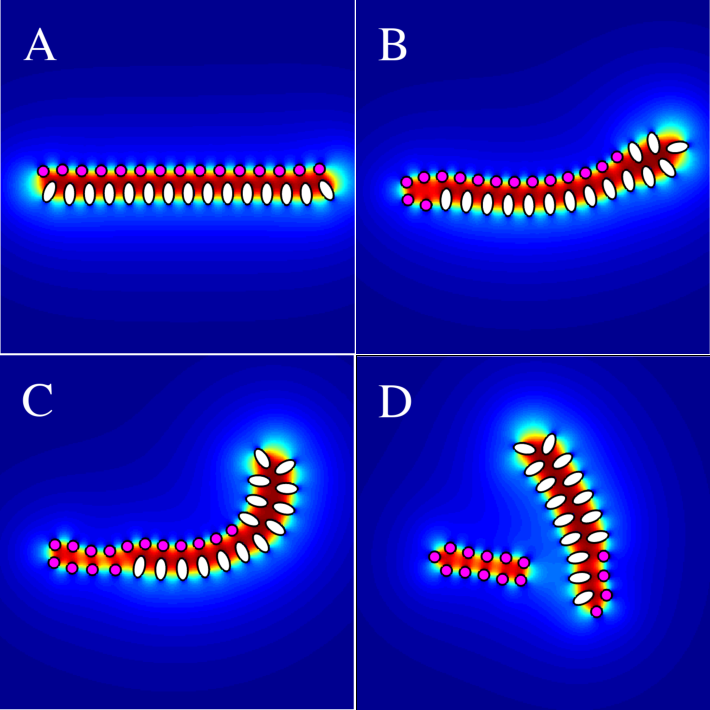
\includegraphics[width=0.4\textwidth]{figures/PW_fig2.pdf}}
%\caption{\label{fig:demixing} An initial assembly of small and 
%large particles spontaneous segregates into two smaller bodies. }
%\end{wrapfigure}
%The HAP simulations show vesicle tank-treading. Under the external shear flow, the initially circular 
%vesicle rotates in the clockwise direction. As the rate of rotation increases, the vesicle approaches
%a steadily tank-treading ellipse. In Figure \ref{fig:tanktreading}B-D, the solid curves are ellipses fit to the particle centers
%and midplane respectively. In the non-dimensionalized system, the particles have diameter 2, on the order of $\rho,$ 
%and the vesicle diameter is about 14. 
%\todo[inline]{missing units. nm?}
%Figure~\ref{fig:tanktreading}E shows the aspect ratio of the major to minor axes reaching an equilibrium value in the 
%red and blue curves, yet oscillating in the high-shear rate (yellow) curve.
%The tank-treading vesicle elongates and becomes more horizontal 
%with an increase in flow rate or 
%with a decrease in stiffness (effected by decreasing $\rho = 4$ to $\rho = 2$). 


%For large shear flow rates, there is an increase in arc length. Here arc
%length refers to the the mid-plane circumference. Thus, some of the
%external force is going into stretching the vesicle---the other part is
%going into bending and viscous dissipation. From our experiments, we
%find that the vesicle ruptures once stretching exceeds about 5 \% (see
%Figure \ref{fig:rupture}). Finally, movies of the tank-treading motion
%show a slip velocity between the outer and inner leaflets Figure
%\ref{fig:tanktreading}G. We have illustrated this by tracking the
%distance between two reference particles in the inner and outer leaflet
%(Figure \ref{fig:tanktreading}B \& D, green and blue particles). With
%moderate shear rates or greater adhesion, the particle pair moves in
%tandem (in Figure \ref{fig:tanktreading}H, blue and red curves, their
%distance is more or less constant). For a large shear rate, the
%particle separates as the two leaflets slide against one another. 

%\begin{figure}
%\begin{center}
%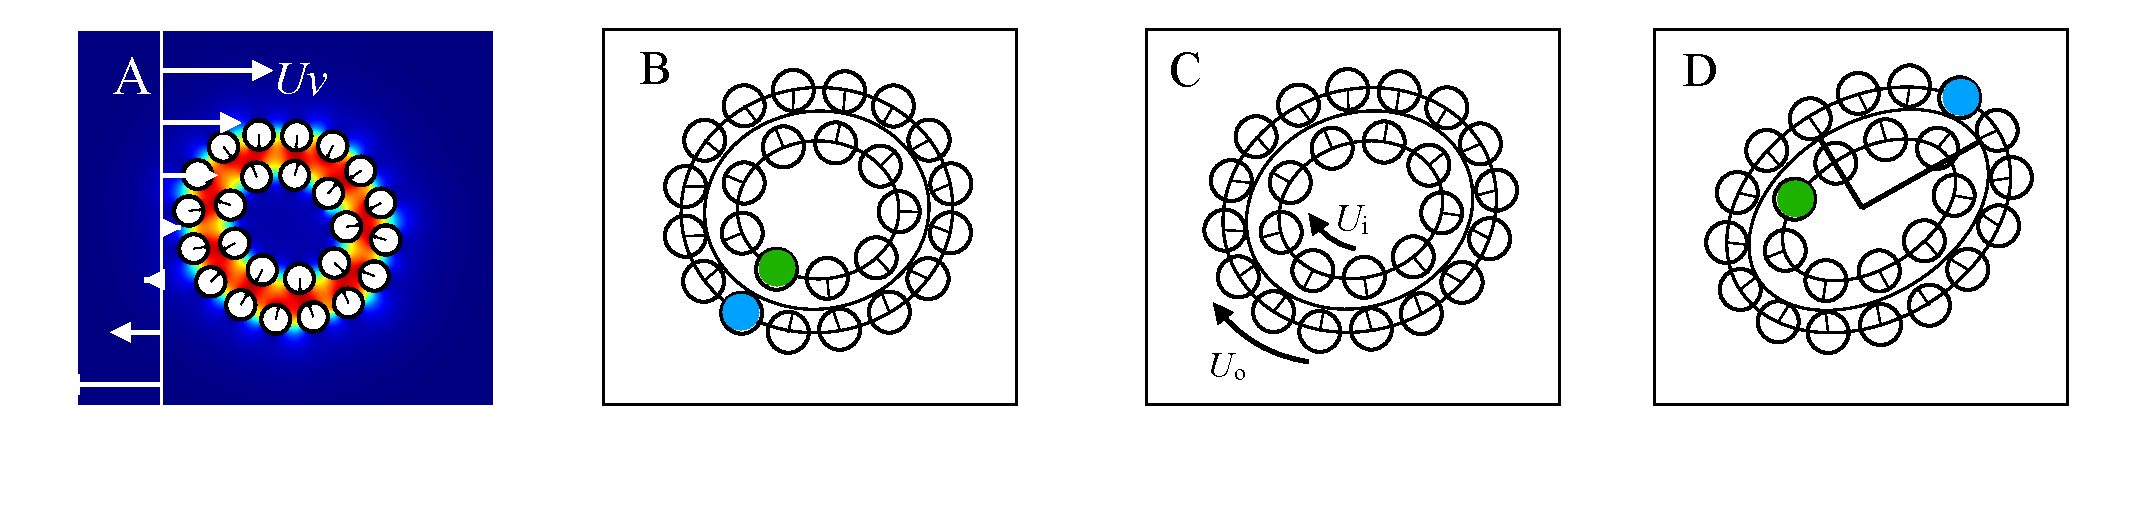
\includegraphics[width=1\textwidth]{figures/PW_fig1A-D.pdf}
%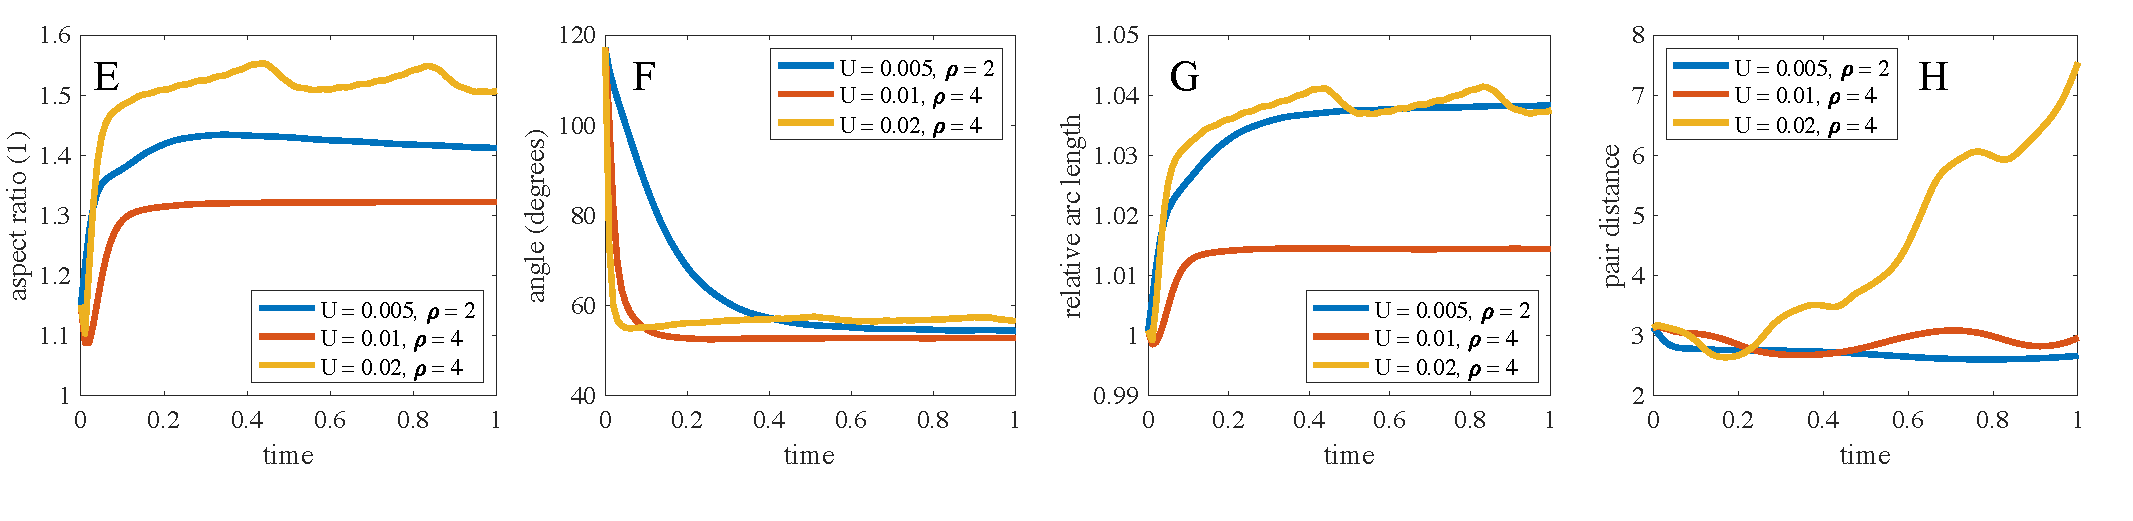
\includegraphics[width=1\textwidth]{figures/PW_fig1E-H.pdf}
%\end{center}
%\vspace{-0.3in}
%\caption{\label{fig:tanktreading}\footnotesize (A) A vesicle formed by
%  amphiphilic particles in shear flow, and the tank-treading motion
%  (B)--(D). The separation of particle pairs in (B) and (C) illustrate
%  inter-leaflet slip.  (E)--(G) Tank-treading reaches a steady state in
%  elliptical aspect ratio, major-axis angle, and circumference.}
%\end{figure}


%\begin{wrapfigure}[12]{r}{0.2\textwidth}
%\centerline{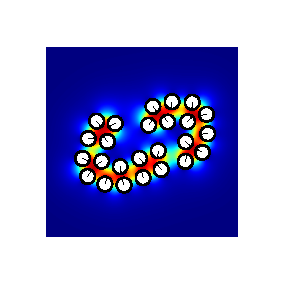
\includegraphics[width=0.2\textwidth]{figures/PW_fig5.pdf}}
%\caption{\label{fig:rupture} Rupture of tank-treading vesicle under strong shear flow.}
%\end{wrapfigure}
%




